\chapter{Architecture}
% OR: \chapter{Model}
\label{cha:architecture}

\begin{comment}
Here you will present the architecture or model that you have chosen and which is (or will be) implemented in your work.
Note that putting algorithms in your report is not always desirable, so in certain cases those might be placed in the appendix.
Code is normally to be avoided in the report itself, but may be included in an appendix or submitted as additional documents.
(The actual code must also be submitted together with the final Master's thesis, but as a zip-file.)

Any off-the-shelf tools and methods that you use in your architecture should have been introduced earlier,
tentatively in the Background chapter (or in the Related Work chapter),
so that they can be referenced here by giving backward pointers to the previous text.

Here, or in a separate chapter (or possibly in the Background chapter or in the Experimental Setup),
you should also discuss the data that you use in your experiments (see Chapter~\ref{cha:data}).

\textit{Nunc in tristique risus, ut malesuada tortor. Integer ullamcorper nunc a felis vehicula condimentum. Aliquam eget turpis purus. Nam nec ipsum sed ligula vulputate tempor ac non arcu. Aenean hendrerit pretium ante et suscipit. Proin vitae venenatis ex, at pellentesque erat. Nulla facilisi. Sed quis eros lorem. Praesent id pharetra risus. Nunc a lacinia est. Nunc in urna at purus ullamcorper blandit eget sit amet est. Cras sagittis et ante ut lobortis. Proin quis arcu eros. Aliquam tempor neque vehicula lacus placerat, ac ultricies massa ultricies. Aliquam et nulla eget felis accumsan rutrum quis sed ligula.}

\textit{Vivamus bibendum tempus tincidunt. Integer imperdiet lectus pellentesque, rhoncus quam at, tempor ex. Phasellus semper tempor sapien at consequat. Proin ut dolor interdum, ullamcorper leo ac, convallis metus. Nullam tincidunt, metus ullamcorper sodales placerat, ipsum ipsum porttitor est, id volutpat orci orci sit amet quam. Vestibulum sagittis urna sit amet nulla vulputate, nec pellentesque enim hendrerit. Suspendisse at laoreet ipsum. Phasellus arcu nisi, laoreet sed tellus sit amet, imperdiet fringilla ante. Quisque rhoncus accumsan magna vel posuere. Fusce facilisis est eros, ac viverra diam maximus ut. Nullam ut lectus nunc. Fusce vestibulum sem at ex euismod tempus. Lorem ipsum dolor sit amet, consectetur adipiscing.}

\textit{Phasellus sed ipsum nunc. Nam iaculis felis mauris, sit amet condimentum ex malesuada at. Morbi lacinia odio mi, sit amet pellentesque ante facilisis sit amet. In lobortis elit ut dictum mollis. Aliquam erat volutpat. Morbi sit amet metus nisi. Nulla auctor varius metus at rhoncus. Pellentesque porta mollis leo, eu ultricies nulla mollis ac. Vivamus interdum ac odio vitae sodales. Aenean finibus eros rhoncus molestie elementum. Integer maximus erat vitae purus lobortis iaculis. Etiam blandit varius nulla, sed euismod felis.}

Clearly, a figure showing the architecture is a must, such as Figure~\ref{fig:Architecture}.
Describe all parts of such a figure in reasonable detail in the text, possibly with forward pointers to sections where they will be elaborated on (or backward pointers to sections where tools and methods already have been introduced).
Mention work that motivated your architectural choices, parameter settings, etc.
Those choices should then also be discussed and elaborated on in the Discussion chapter.

\begin{figure}[t!]
    \centering
    \missingfigure{Architecture figure to be added}
    \caption{The missing architecture}
    \label{fig:Architecture}
\end{figure}
\end{comment}

\section{High-Level Application Architecture}

A microservice architecture was employed in order to simplify development and separate concerns between the different microservices. The services are deployed as Docker Containers, and they are orchestrated using Docker Compose. \todo{quickly explain docker and why it is useful here} \autoref{fig:architecture-overview} shows how the application is divided into five distinct services, and the direction of information flow between these.

\begin{figure}[h]
    \centering
    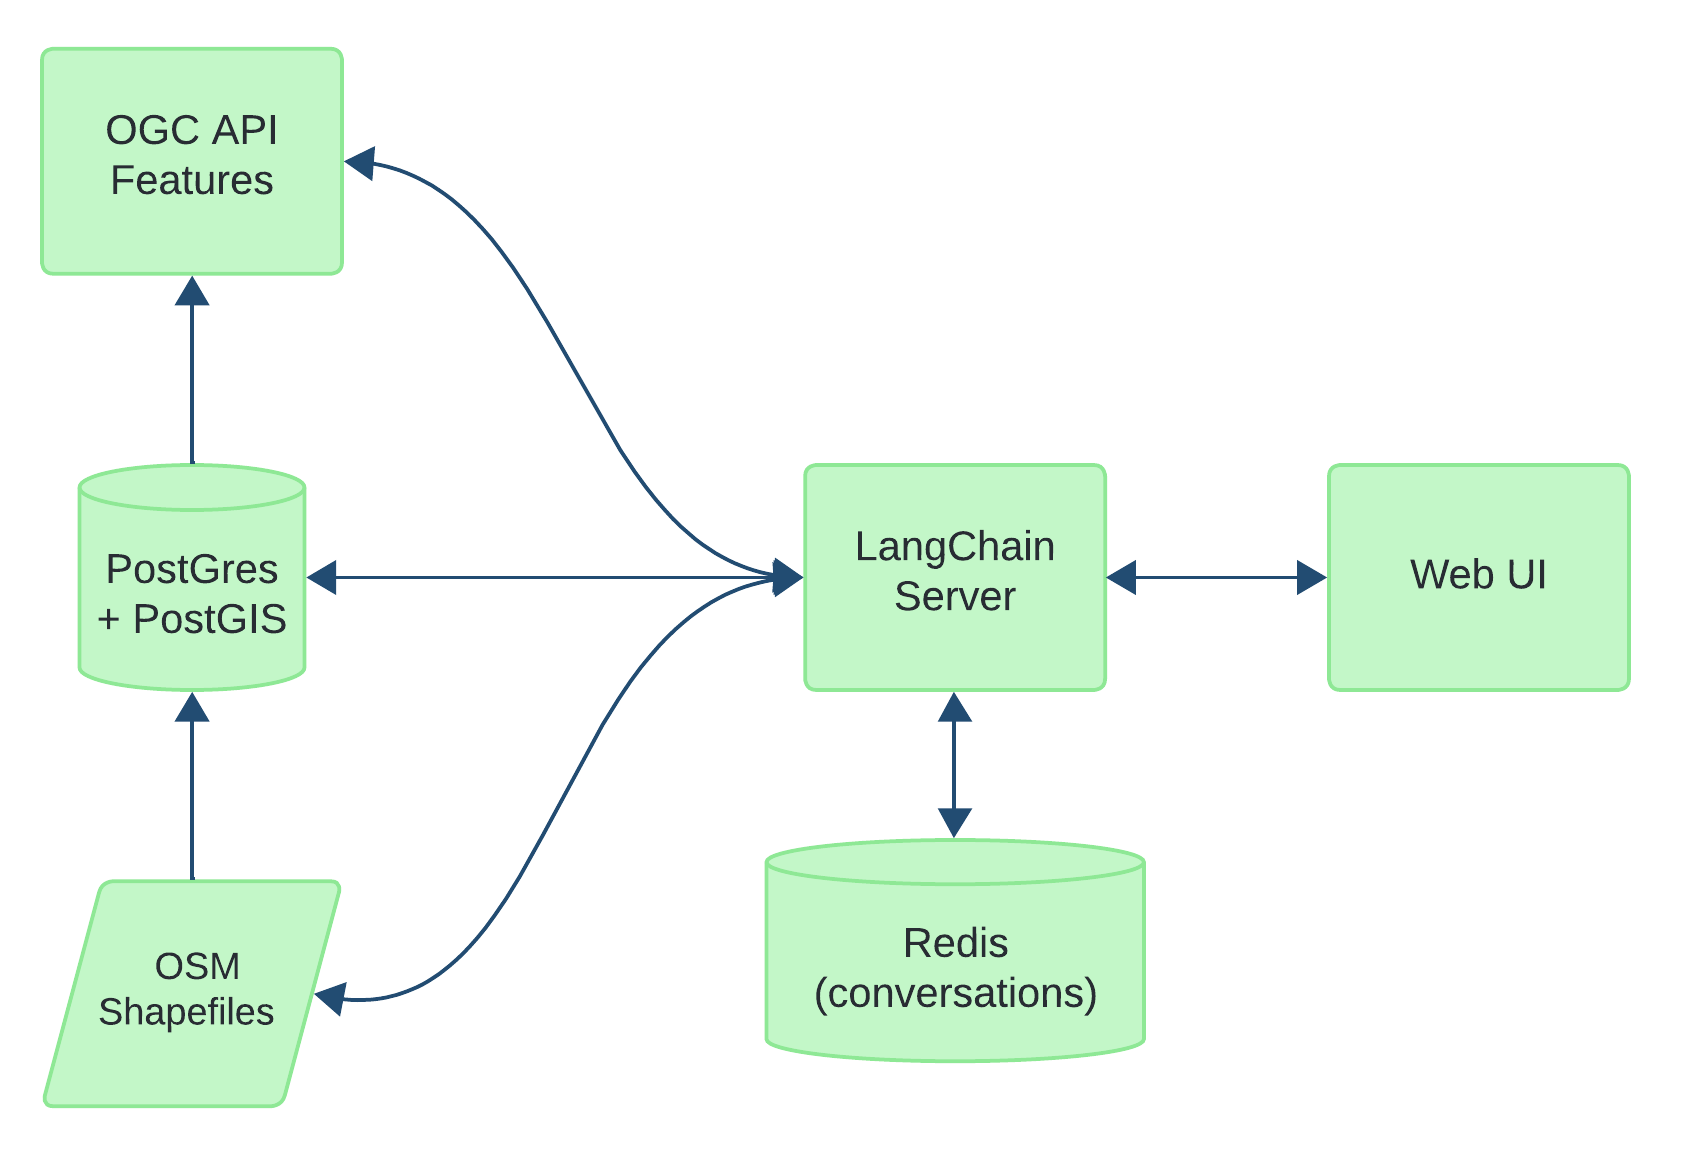
\includegraphics[width=\textwidth]{microservices.png}
    \caption{Architecture overview}
    \label{fig:architecture-overview}
\end{figure}



\subsection{LangChain Server}\label{subsec:langchain}

The \textit{LangChain Server} service is the heart of the application, and is where the \gls{acr:llm}-related logic is situated. It is responsible for taking requests from the \textit{Web \acrshort{acr:ui}} and returning suitable responses in what becomes a client-server architecture between the two services. \autoref{tbl:server-endpoints} show the endpoints exposed by the server and how they can be used by a client.

\begin{table}[h]
    \centering
    \caption{Summary of Server Endpoints}
    \label{tbl:server-endpoints}
    \begin{tabular}{p{0.22\textwidth}p{0.1\textwidth}p{0.55\textwidth}}
        \toprule
        \textbf{Endpoint} & \textbf{Method} & \textbf{Description}                                                                                                                                                         \\
        \midrule
        /session          & GET             & Takes a \texttt{session\_id} as a query parameter, allowing the client to continue on a pre-existing session.                                                                \\
        /session          & POST            & Creates a new session with an empty conversation.                                                                                                                            \\
        /streaming-chat   & GET             & Endpoint for chatting the \acrshort{acr:llm}. Takes a \texttt{message} as a query parameter and returns an event stream, allowing for token streaming from server to client. \\
        /update-map-state & POST            & Send the state of the client map to the server. Keeps the server updated on what layers are present in the map, their color, etc.                                            \\
        /geojson          & GET             & Takes a \texttt{geojson\_path} as a query parameter. Allows the client to retrieve a given GeoJSON file that is stored in the working directory on the server.               \\
        /history          & GET             & Used to retrieve the chat history of the current session.                                                                                                                    \\
        /upload           & POST            & Allows the client to upload one or more files to the working directory on the server.                                                                                        \\
        \bottomrule
    \end{tabular}
\end{table}


\subsection{Redis for Conversations}

Redis \citep{sanfilippoRedisRealtimeData2009} is a fast in-memory database that is often applied as a caching database that sits on top of some persistent database. It can also be used for vector-based storage and as a simple NoSQL database. The latter option is the way it is used in GeoGPT's architecture, and its only purpose is to store conversations. Whenever a user starts a conversation with GeoGPT an object with a unique session ID is stored to the Redis database. This object holds an array that represents the conversation. This array is written to every time either the human or GeoGPT produces a message.

Storing messages --- either in memory as a simple array or in a database like Redis --- is crucial to enable multi-message conversations. In order for a \gls{acr:llm} to act as a conversational agent, some sort of chat history needs to be prepended to the prompt. In the case of GeoGPT the entire chat history is prepended. This has the advantage of providing the \gls{acr:llm} with the complete context of the chat history, but the disadvantage of potentially bloating the context window from which it is supposed to generate tokens. Therefore, as the chat becomes longer each new token will be both more expensive and take more time to get generated. A long chat history could also make the resulting prompt exceed the token limit of the \gls{acr:llm}, or it could confuse model by providing it with messages no longer relevant to the conversation. These issue was not considered in great detail for this project, and are left for future work.

\subsection{PostGres + PostGIS}



\subsection[OGC API Features]{\acrshort{acr:ogc} \acrshort{acr:api} Features}

On top of the PostGIS database  containing \gls{acr:osm} data is a RESTful geospatial feature server called \textit{pg\_featureserv} \citep{crunchydataCrunchyDataPg_featureserv2024}.


\subsection[Web UI]{Web \acrshort{acr:ui}}

The user interface is made with SolidJS. By design, it is very minimal. One of the goals of the project is to simplify the way we do \acrshort{acr:gis} analysis. One of the key design goals was therefore to make the interface as familiar to the user as possible and lowering the chance of the user doing something wrong. The chat interface was designed to imitate the interface of OpenAI's

\begin{figure}[h]
    \centering
    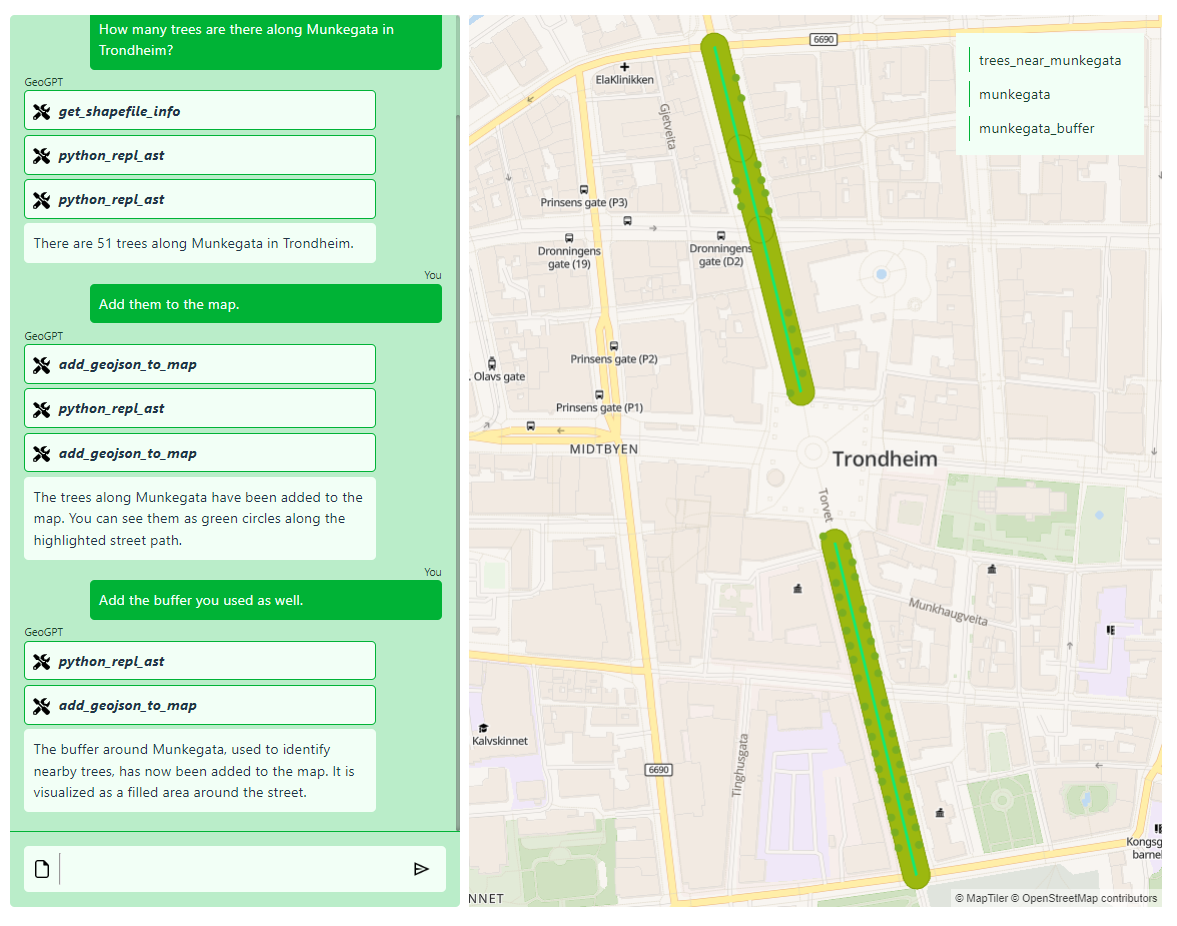
\includegraphics[width=\textwidth]{num_trees_along_munkegata_python_with_buffer.png}
    \caption{Web \acrshort{acr:ui}}
    \label{fig:web-ui}
\end{figure}


\glsresetall



\section{Agent Architectures}

\subsection{LangGraph Agent Implementation}

\subsection{Prompt Templating}

\subsection{Tools}

